\chapter[Proposed Methodology/Approach]{Proposed Methodology/Approach}{Proposed Methodology/Approach}\label{pm}

\rule{0.49\textwidth}{0.75pt} $_{\bigcirc}$ \rule{0.49\textwidth}{0.75pt}\\
\section{Problem Definition}
Under the present digital ecosystem, the process of identity verification has people sharing all the government documentation of their identity with several platforms including telecom, banking and government services. This results in unjustified sharing of sensitive personal information such as address, UID and personal contacts, without necessarily the user knowing how their data is stored or utilized. Current systems emphasize on secure storage and transfer but continue to use data visibility on verification. This brings about the danger of misuse, fraud and unauthorized access, as demonstrated in real world cases. It is necessary to have a system that checks the authenticity of the user without revealing personal information and ensuring security, user control and trust. Controlled access, revocation and interoperability to current infrastructures should also be supported by such a system. This secures realistic adoption, and high privacy and security levels. It must reduce reliance on centralized authorities and provide reliable and tamper resistant verification.




\section{Objectives}
 \begin{enumerate}
  \item Make sure Privacy Preserving Identity Verification:
  \begin{enumerate}
    \item Support users to authenticate themselves without showing personal information with Zero Knowledge Proofs.
    \item Do away with the necessity to disseminate raw government ID documents on several platforms.
  \end{enumerate}
  
  \item Secure Data Storage of Identity:
  \begin{enumerate}
    \item Hash user identity documents of stores in IPFS with cryptographic hashing to ensure integrity and security.
  \end{enumerate}
  
  \item Enhance Access Control Measures:
  \begin{enumerate}
    \item  Introduce role based access control by smart contracts to make secure verification requests.
    \item Enable users to give, deny and take away permission to their identity data.
  \end{enumerate}
  
  \item Leverage Decentralized Technologies:
  \begin{enumerate}
    \item Implement blockchain, Self Sovereign Identity and ZK STARK to ensure safe and transparent authentication.
    \item Decentralized identifiers and verifiable credentials: User controlled identity management using decentralized identifiers and verifiable credentials.
  \end{enumerate}
  
  \item Promote User Ownership and Recovery:
  \begin{enumerate}
    \item  Add the feature of a guardian based wallet recovery, to avoid irreversible loss of user access.
    \item  Have complete ownership of identity data without being reliant on centralized authorities.
  \end{enumerate}
  
  \item Make Real World Integration possible:
  \begin{enumerate}
    \item Design the system to work alongside existing platforms like DigiLocker and Aadhaar services.
    \item Scale up adoption of government, telecom, business and enterprise verification systems.
  \end{enumerate}
\end{enumerate}


\section{Scope}
TrustChain concentrates on the reinvention of identity verification by adding a privacy preserving layer to the current digital systems. It will minimize the reliance on the provision of full identity documents in various platforms like banking services, telecommunication, and government services. The system facilitates a higher level of trust and security in digital interactions by using decentralized technologies that ensure that verification is conducted on the basis of proof instead of exposing data, which enhances overall trust and security in digital interactions.

The project will also be developed to be connected with the existing infrastructures, such as DigiLocker and Aadhaar based services, without substituting them. It facilitates secure onboarding, decentralized storage via IPFS and proves via ZK STARK. Role based access control is also facilitated by the system which allows users to control access, grant and revoke access where necessary. This grants flexibility and control whilst being compatible with real world applications and workflows.

The scope also touches on improving user ownership through the addition of features such as guardian based wallet recovery, and decentralized identifiers. It is concerned with the construction of a system in which the users are in full control of their identity data without the need to have centralized bodies control and access their identity data. The scope also extends to the improvement of user ownership such as the addition of features such as guardian based wallet recovery and decentralized identifiers. 

The project can be scaled up in the future to enable large scale implementation both in the public and the private sectors. It may be connected to the government databases to verify authenticity and may be extended with the simplified user interfaces to allow the system to be used by non technical users. The project can be scaled up in the future to enable big adoption in the public and private sector. It can be incorporated with government databases to check authenticity and extended with simplified user interfaces to enable non technical users to use the system. 



\section{Proposed Approach}
The TrustChain approach that is proposed is aimed at the creation of a privacy preserving identity verification system with the help of decentralized technologies. It makes sure that the users do not have to present their full identity document to get verified. Rather, the system authenticates authenticity by using cryptographic evidence, and ensures confidentiality but can allow access to be safe and trusted across a variety of digital environments.

The system starts by registering users where people create an account and add various guardian wallet addresses which they use in case of recovery. Users can then upload their government identity documents once, which are stored in IPFS in a secure manner. Each document is given a unique cryptographic hash guaranteeing integrity and thwarting any unethical alteration or reproduction throughout the ecosystem.

To verify identity, the system is based on the principles of Self Sovereign Identity with Zero Knowledge Proofs. The input to the proof generation process is in the form of documents, which enable users to show authenticity without showing the real information. ZK STARK supports more security through the use of hash mechanisms that minimize risks with traditional cryptographic methods and provide assured verification.

The blockchain has smart contracts that validate identity and provide role based access control. When a requester makes a verification request, permission assessment and generation of responses in the form of proof is done by the system rather than the exchange of documents. Users are also in full control of giving, denying or revoking access any time, so that identity usage is transparent, controlled and in line with user consent.

Comprehensively, the strategy will guarantee that the process of identity verification is converted into a proof based mechanism in lieu of a data sharing process. Embracing blockchain, IPFS, SSI and ZK STARK, TrustChain offers a secure and scalable system that ensures the privacy of users and supports trust and efficiency in the real world identity verification settings. Further, it allows users to have full control of their information regarding identity data by allowing permission based access and revocation when necessary. The system also minimizes reliance on centralized authorities and also remains reliable and therefore can be integrated with the existing digital infrastructures. It further establishes a standardized approach for privacy focused identity.

\subsection{Proposed System Architecture}

\begin{figure}[h!]
    \centering
    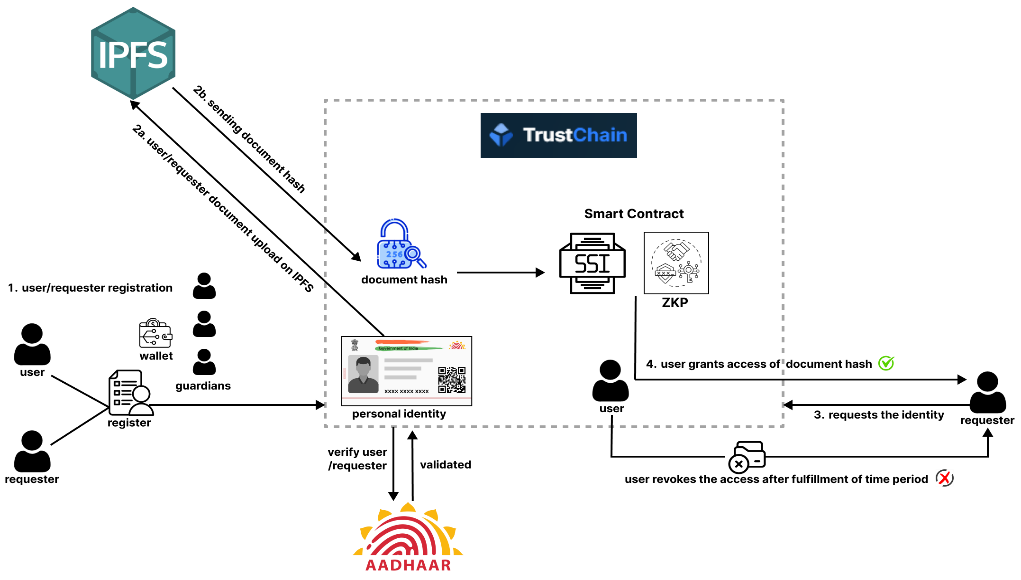
\includegraphics[width=1\textwidth]{Chapter1/trustchain_architecture.png} % Adjust the width as needed
    \caption{TrustChain Framework Architecture}
    \label{f1} % Optional: for referencing the figure in your document
\end{figure}


TrustChain framework is developed as a fully user centric identity life cycle that is privacy, control and secure verification oriented. The architecture allows identity not to be revealed in crude form but instead facilitates the verification to occur effectively. This is a system that is based on the decentralized technologies which use the combination of blockchain and IPFS, Self Sovereign Identity and Zero Knowledge Proofs. It brings in an ordered sequence of activities, starting with safe onboarding, then credential storage, hashing, verification and access control. There is an attention to each stage where it is designed to remove the redundant data sharing with integrity and trust. The architecture also makes sure that the users are in complete control of their identity during the process. The framework solves the major problems of misuse of data and unauthorized exposure of data in current systems by moving away the traditional document based verification into the proof based verification. It also develops a generalized flow which can be embraced in various fields. The modular design enables an easy extension and upgrade in the future. The system design will have the ability to be compatible with the emerging digital identity standards. This renders the architecture to be scalable and suitable to long term use.

The system starts by having a user registration process which is non redirectional making the on boarding process smooth. Users are expected to put in three guardian wallet addresses during registration that are used as recovery agents. Such guardians are significant in the recovery of the accounts in case they get lost. This ensures that it is not highly reliant on centralized recovery systems. It also enhances trust because recovery is spread among the entities that are trusted. The onboarding is maintained simple so as to make it easy to use. This enhances its adoption by non technical users also.


After the registration process, the system first does initial verification and safely creates a master private key to the user. This key is shared with the individual and is the central control and authentication mechanism among the platform. The key will make sure that verification actions can only be taken by the owner. Key handling practices need to be properly applied to ensure security. This enhances the authentication system of the system. It also complies with the decentralized identity ownership principles.

Following the onboarding, the users post their government identity documents to the platform. They are stored in IPFS as PINATA that provides a decentralized and safe storage. IPFS assigns a content identifier to every document that serves as the foundation of additional cryptographic processes in the system. This eliminates the necessity to have centralized stores. It enhances fault tolerance and availability too. Information in the form of documents cannot be easily accessed by mere queries. This guarantees an added level of security.

To increase the level of security, the IPFS generated hash is subjected to another round of hashing with keccak256. This hash is then hashed again, to make sure it is irreversible. This hybrid hash method ensures that there is no chance of restoring the original document and at the same time be able to check the integrity. It enhances opposition to brute force attacks. The stacked hashing structure makes life more difficult on the part of attackers. This guarantees security as opposed to single hash systems. It is also efficient in the verification operations.

The identity verification is developed based on the principles of Self Sovereign Identity where a user has control over his or her data. There is limited information that is shared like name, email and date of birth. Checking is done through the Zero Knowledge Proofs that verify authenticity without exposing sensitive information. This will minimize unnecessary exposure of data when it is verified. It provides adherence to privacy oriented needs. Access duration can be defined depending on the need of the users. This provides full freedom in the use of identities.

ZK STARK is utilized when generating proofs since it is based on hash functions and does not require the trusted setup. It makes it more resistant to attacks, e.g. replay or inference attempts. The verification process is used to compare the calculated hashes with the stored values on chain to confirm the authenticity of the identity. This enhances trust on the verification outcomes. It minimizes the need to rely on third party validation systems. The generation of proof can be done in adversarial conditions as well without being compromised. This renders the system strong to be used in the real world.

The entire access control mechanism is controlled by smart contracts deployed with Solidity on the OP Sepolia Testnet. They give requesters merely demonstrations of validity as opposed to real documents. Users have the permission to give, deny or take back access anytime and everything is documented on the blockchain ensuring transparency, security and applicability in real world domains. This leaves a permanent chronicle of all the activities. It makes sure that there is accountability of each access request. The system does not deal with any form of financial transactions to ensure that it does not lose sight of identity checking. This makes the architecture very straightforward and functional.




\rule{0.49\textwidth}{0.75pt} $_{\bigcirc}$ \rule{0.49\textwidth}{0.75pt}\\
